% V6 paper-geometry typography preview (10pt two-column IEEEtran).
% Figures only — does not modify manuscript prose.
\documentclass[journal,10pt,twocolumn]{IEEEtran}
\usepackage[T1]{fontenc}
\usepackage[utf8]{inputenc}
\usepackage{graphicx}
\usepackage{subcaption}
\usepackage{microtype}

% Symlinks under _preview_links avoid spaces in PDF paths.
\graphicspath{{_preview_links/}}

\title{V6 Camera-Ready Figure Typography Preview}
\author{MD2G ToN Figure Pipeline}
\date{}

\begin{document}
\maketitle

\begin{abstract}
Typography audit only: MAIN\_TEXT figures at planned inclusion widths under IEEEtran 10pt twocolumn.
\end{abstract}

\section{FIGURE A --- Overall + scaling}
\begin{figure*}[!t]
\centering
\begin{subfigure}[t]{0.48\textwidth}
\centering
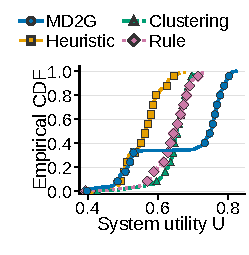
\includegraphics[width=\linewidth]{QoE/QoE_By_Strategy.pdf}
\caption{ECDF of system utility $U$.}
\end{subfigure}\hfill
\begin{subfigure}[t]{0.48\textwidth}
\centering

\includegraphics[width=\linewidth]{Buffer/System_Utility_By_Users_scheme1.pdf}
\caption{Mean $U$ vs concurrency.}
\end{subfigure}
\caption{Overall distribution and concurrency scaling.}
\end{figure*}

\section{FIGURE B --- Robustness}
\begin{figure*}[!t]
\centering
\begin{subfigure}[t]{0.48\textwidth}
\centering
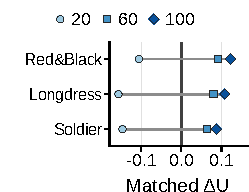
\includegraphics[width=\linewidth]{QoE/QoE_By_Content_DeltaU.pdf}
\caption{Matched $\Delta U$ by content $\times$ load.}
\end{subfigure}\hfill
\begin{subfigure}[t]{0.48\textwidth}
\centering
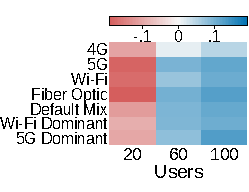
\includegraphics[width=\linewidth]{QoE/QoE_By_Network.pdf}
\caption{Matched $\Delta U$ by network $\times$ load.}
\end{subfigure}
\caption{Robustness across content and access profiles.}
\end{figure*}

\section{FIGURE C --- Holdout + mechanism}
\begin{figure*}[!t]
\centering
\begin{subfigure}[t]{0.48\textwidth}
\centering
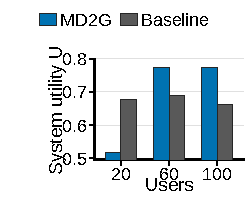
\includegraphics[width=\linewidth]{QoE/Loot_Holdout_DeltaU_By_Users.pdf}
\caption{Matched utility on the unseen Loot holdout. MD2G trails the strongest same-substrate baseline at 20 users but leads at 60 and 100 users.}
\end{subfigure}\hfill
\begin{subfigure}[t]{0.48\textwidth}
\centering
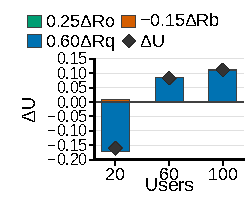
\includegraphics[width=\linewidth]{QoE/Mechanism_Decomposition_Loot.pdf}
\caption{Utility decomposition (not an ablation).}
\end{subfigure}
\caption{Holdout transfer and measured utility components.}
\end{figure*}

\section{FIGURE D --- Architecture}
\begin{figure*}[!t]
\centering
\begin{subfigure}[t]{0.48\textwidth}
\centering
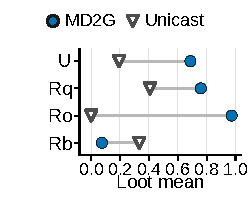
\includegraphics[width=\linewidth]{QoE/MoQ_Shared_vs_Unicast.pdf}
\caption{Shared MoQ vs MoQ-Unicast.}
\end{subfigure}\hfill
\begin{subfigure}[t]{0.48\textwidth}
\centering

\includegraphics[width=\linewidth]{UX/H2_Cross_Stack_DASH.pdf}
\caption{Cross-stack utility comparison at 20 and 60 users. MD2G outperforms GROOT and Rolling, but the result reflects end-to-end system differences.}
\end{subfigure}
\caption{Architecture and secondary cross-stack comparison.}
\end{figure*}

\section{FIGURE E --- Representative physical load (shared legend)}
\begin{figure*}[!t]
\centering
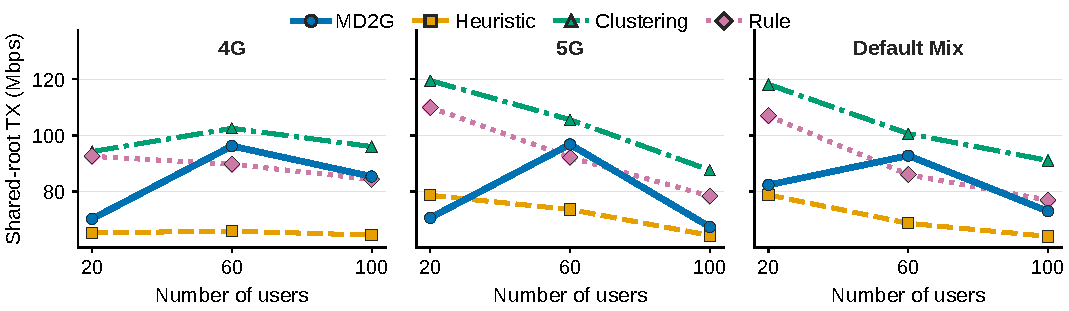
\includegraphics[width=\textwidth]{Throughput/System_Throughput_MainText_1x3.pdf}
\caption{Shared-root TX under 4G, 5G, and Default Mix. Supporting load evidence only: lower TX is not higher efficiency.}
\end{figure*}

\section{Optional Discussion --- Rb--U operating points}
\begin{figure*}[!t]
\centering
\begin{subfigure}[t]{0.32\textwidth}
\centering

\includegraphics[width=\linewidth]{UX/TierB_Rb_vs_U_4G.pdf}
\caption{4G.}
\end{subfigure}\hfill
\begin{subfigure}[t]{0.32\textwidth}
\centering

\includegraphics[width=\linewidth]{UX/TierB_Rb_vs_U_5G.pdf}
\caption{5G.}
\end{subfigure}\hfill
\begin{subfigure}[t]{0.32\textwidth}
\centering

\includegraphics[width=\linewidth]{UX/TierB_Rb_vs_U_Default_Mix.pdf}
\caption{Default Mix.}
\end{subfigure}
\caption{Operating-point visualization ($R_b$ vs $U$). Supporting only; $U$ already includes $-0.15 R_b$.}
\end{figure*}

\end{document}
